\documentclass[prd,reprint,nofootinbib,notitlepage,aps,tightenlines,amsmath,amssymb,showpacs,superscriptaddress]{revtex4-1}
\usepackage[hyperindex,breaklinks]{hyperref}
\usepackage{graphicx,epstopdf}
%\usepackage{subfig}
\usepackage{tikz}
\usepackage{amsmath}
\usetikzlibrary{shapes,arrows}
%\usepackage{subfig}
\usepackage{mathtools}
%\usepackage{feynman}
\usepackage{subfigure}

\usepackage{natbib,bm}
%
\usepackage{slashed}    
\usepackage{hyperref}
\usepackage{breakurl}
\usepackage{multirow}
\usepackage{bbold}
\usepackage{listings}
\usepackage{booktabs}

\usepackage{soul}

\def\simgt{\mathrel{\raise.3ex\hbox{$>$\kern-.75em\lower1ex\hbox{$\sim$}}}}
\def\simlt{\mathrel{\raise.3ex\hbox{$<$\kern-.75em\lower1ex\hbox{$\sim$}}}}

%\newcolumntype{C}{>{$}c<{$}}
\AtBeginDocument{
\heavyrulewidth=.08em
\lightrulewidth=.05em
\cmidrulewidth=.03em
\belowrulesep=.65ex
\belowbottomsep=0pt
\aboverulesep=.4ex
\abovetopsep=0pt
\cmidrulesep=\doublerulesep
\cmidrulekern=.5em
\defaultaddspace=.5em
}
\lstset{
basicstyle=\small\ttfamily,
columns=flexible,
breaklines=true
}

%%%%%%%%%%%%%%%%%%%%%%%%%%%%%%%%%%%%%%%%%%%%%%%%%%%%%%%%%%%%

\begin{document}
\title{Signal sample generation for stop four body decays}
\author{Suchita Kulkarni}
%\affiliation{Institute of High Energy Physics, Austrian
%     Academy of Sciences, Nikolsdorfergasse 18, 1050 Vienna,
%     Austria}
\email{suchita.kulkarni@gmail.com}     
%%%%%%%%%%%%%%%%%%%%%%%%%%%%%%%%%%%%%%%%%%%%%%%%%%%%%%%%%%%%
\begin{abstract}
\noindent 

\end{abstract}
%%%%%%%%%%%%%%%%%%%%%%%%%%%%%%%%%%%%%%%%%%%%%%%%%%%%%%%%%%%%
\maketitle
\onecolumngrid
%%%%%%%%%%%%%%%%%%%%%%%%%%%%%%%%%%%%%%%%%%%%%%%%%%%%%%%%%%
%%%%%%%%%%%%%%%%%%%%%%%%%%%%%%%%%%%%%%%%%%%%%%%%%%%%%%%%%
%%
\section{Introduction}
%%%%%%%%%%%%%%%%%%%%%%%%%%%%%%%%%%%%%%%%%%%%%%%%%%%%%%%%%%%%
This note describes the status of generator level study of analysis in single displaced lepton final state. The signal model under consideration is stop pair production with small stop - LSP mass splitting. The small mass splitting between the stop and the LSP leads to four body decay of stop and in particular due to suppressed phase space can also lead to long lived stops. We describe here, potential reach of an analysis for such long lived stop via searching for a single displaced electron or muon along with an ISR jet. 

The complication arises with the knowledge that stop two body decay mode with charm and LSP final state has more favoured phase space and thus special theory construction is needed in order to suppress this decay mode. We take~\cite{Grober:2014aha} to be the base theory study where the authors show theory scenarios under which one could obtain long lived stops. Using this as a motivation, we then construct an approximate grid to perform sensitivity analysis. 

Along with the potential reach of the analysis, we also discuss potential reweighting procedure in the stop branching ratio and stop lifetime dimension. 

In technical terms, this sets up the procedure to generate signal samples. In order to increase the efficiency, the pythia fragments are equipped with generator level filters. This note also ships together with existing analysis code which then employees generator level cuts on the final state objects and is also capable of performing reweighting in branching ratio and lifetime dimension. 
%%%%%%%%%%%%%%%%%%%%%%%%%%%%%%%%%%%%%%%%%%%%%%%%%%%%%%%%%%%%
\section{Normalization of samples}
%%%%%%%%%%%%%%%%%%%%%%%%%%%%%%%%%%%%%%%%%%%%%%%%%%%%%%%%%%%%
The samples are normalized to the number of events in single lepton ($e$ or $\mu$) final states. Given the stop production cross section $\sigma^{\tilde t_1}$, the normalization can be obtained as follows: 
\begin{equation}
    \mathcal{N} = \mathcal{L}\times \sigma^{\tilde t_1}\times(2\times\mathcal{BR}(\tilde t_1 \rightarrow b W^*) \times\mathcal{BR}(W\rightarrow l \nu) - \mathcal{BR}^2(\tilde t_1 \rightarrow b W^*) \times\mathcal{BR}^2(W\rightarrow l \nu))\times \epsilon^{\rm{filter}}
\end{equation}

We have taken $\mathcal{BR}(W^*\rightarrow l \nu) = 0.2$ summing over electron and muon final state. Please note, the associated analysis specifically looks for the electrons and muons originating from W decay. For results in this note, the luminosity $\mathcal{L}$ is set to 1 fb$^{-1}$. 
%%%%%%%%%%%%%%%%%%%%%%%%%%%%%%%%%%%%%%%%%%%%%%%%%%%%%%%%%%%%
\section{Full grid}
%%%%%%%%%%%%%%%%%%%%%%%%%%%%%%%%%%%%%%%%%%%%%%%%%%%%%%%%%%%%
In a real life situation, the stop decays via either two or four body final states. As shown in~\cite{Grober:2014aha}, the stop - LSP mass difference, the stop four body final ratio and the stop lifetime are all correlated once the flavour violation co-efficient is fixed. 

Therefore we generate one sample grid as shown in fig.~\ref{fig:prop_grid}, which results from a fixed flavour violating co-efficient. In this case, the stop - LSP mass difference fixes all other parameters of the model. We generate this grid for four stop masses of 200, 300, 400, 500 GeV. We show the results in fig.~\ref{fig:full_grid_dxy02} and fig.~\ref{fig:full_grid_dxy10}. In order to arrive at these results, the following cuts have been employed
\begin{itemize}
    \item $\textrm{MET} > 200 $ GeV
    \item $H_T > 300$ GeV
    \item $p_T(j_1) > 100 $ GeV 
    \item $p_T(j_2) > 50 $ GeV 
    \item $\Delta \phi(j_1, j_2) > 2.5$
    \item $p_T(\mu) > 3.5, |\eta| < 2.4, p_T(e) > 5, |\eta| < 2.5, L_{xy}(e) < 5$ cm
    \item at least one lepton in $0.2\, \textrm{cm} < d_{xy} < 1\, \textrm{cm} $
    \item at least one lepton in $1\, \textrm{cm} < d_{xy} < 10\, \textrm{cm} $
\end{itemize}

We define the $\epsilon_{cut}$ as the efficiency for that particular cut with respect to the initial number of events after filter (and matching).

As can be seen from both figures, the primary message is that the efficiency is almost independent of the stop mass. This can be understood because the analysis is not actually sensitive to any final states. Since the analysis is monojet-like, the efficiencies are not a function of the stop mass. The efficiencies do depend on the stop lifetime and hence on the stop - LSP mass difference. 
%%%%%%%%%%%%%%%%%%%%%%%%%%%%%%%%%%%%%%%%%%%%%%%%%%%%%%%%
\begin{figure}[tb]
%\subfloat{%
  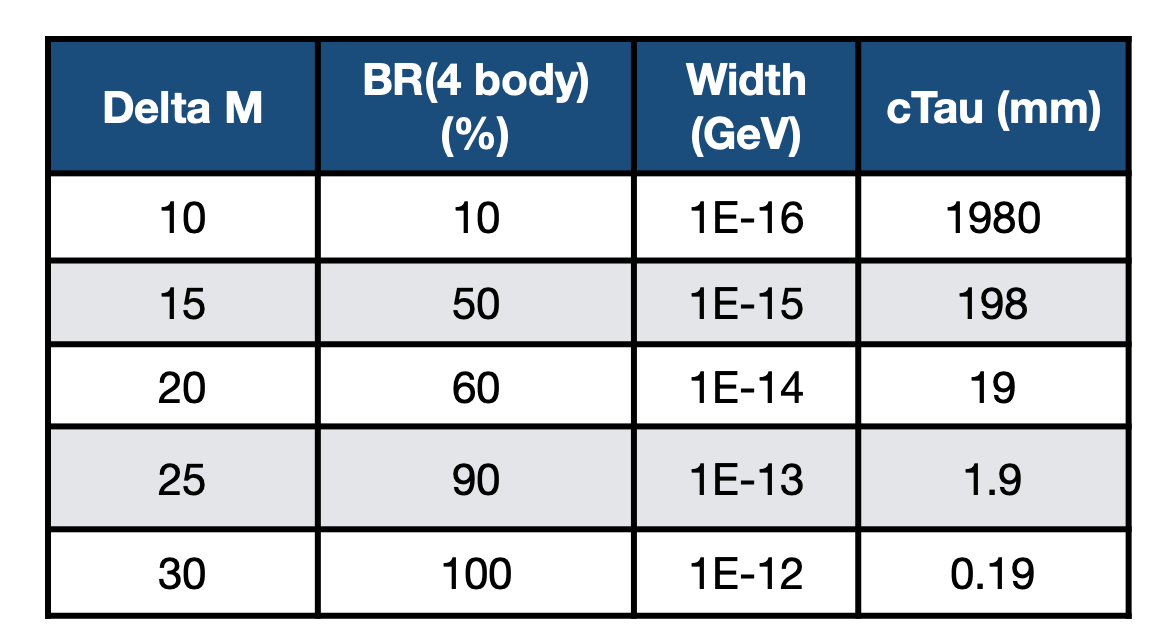
\includegraphics[width=0.7\columnwidth]{./figures/proposed_grid.png}%
 \caption{Parameters of full model where branching ratio, mass different and lifetimes are correlated. This is only one realisation and branching ratio should be varied according to the theory study in~\cite{Grober:2014aha}.}
\label{fig:prop_grid}
\end{figure}
%%%%%%%%%%%%%%%%%%%%%%%%%%%%%%%%%%%%%%%%%%%%%%%%%%%%%%%%%%%%

%%%%%%%%%%%%%%%%%%%%%%%%%%%%%%%%%%%%%%%%%%%%%%%%%%%%%%%%
\begin{figure}[tb]
%\subfloat{%
  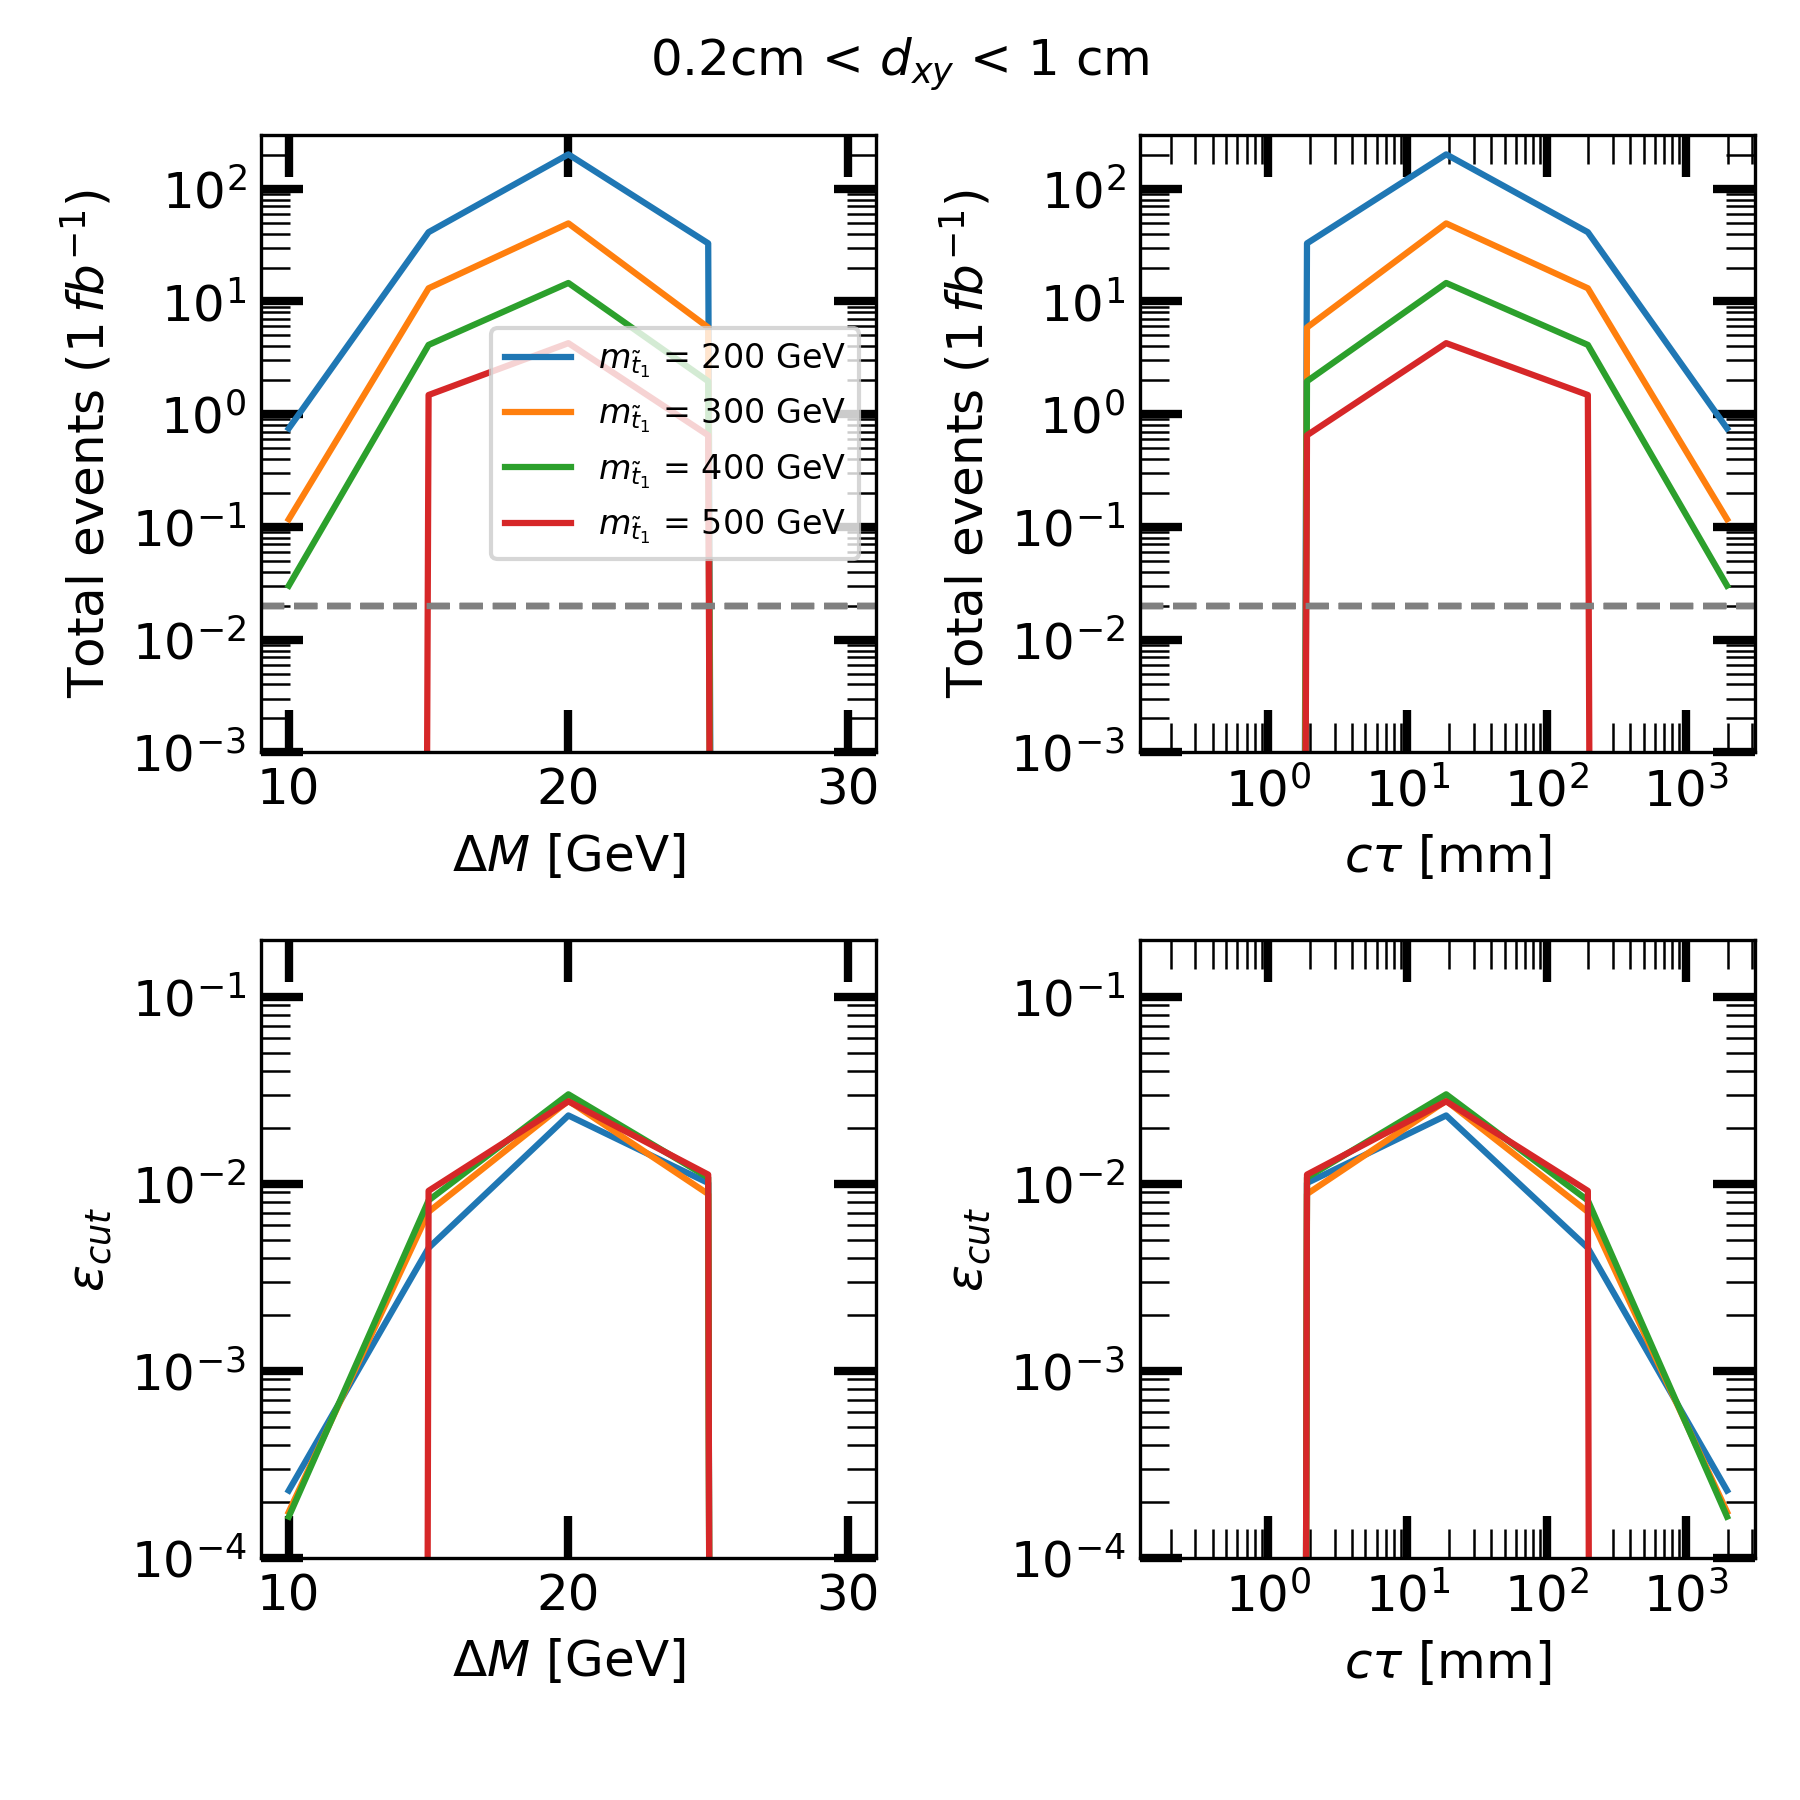
\includegraphics[width=0.8\columnwidth]{./figures/02_dxy_1_full_grid.png}%
 \caption{Sensitivity analysis for full model in the signal region $0.2 cm < d_{xy} < 1 cm$. Top panel shows number of events as a function of $\delta M$ and $c\tau$, while the bottom panel shows efficiency as a function of the same two variables.}
\label{fig:full_grid_dxy02}
\end{figure}
%%%%%%%%%%%%%%%%%%%%%%%%%%%%%%%%%%%%%%%%%%%%%%%%%%%%%%%%%%%%


%%%%%%%%%%%%%%%%%%%%%%%%%%%%%%%%%%%%%%%%%%%%%%%%%%%%%%%%
\begin{figure}[tb]
%\subfloat{%
  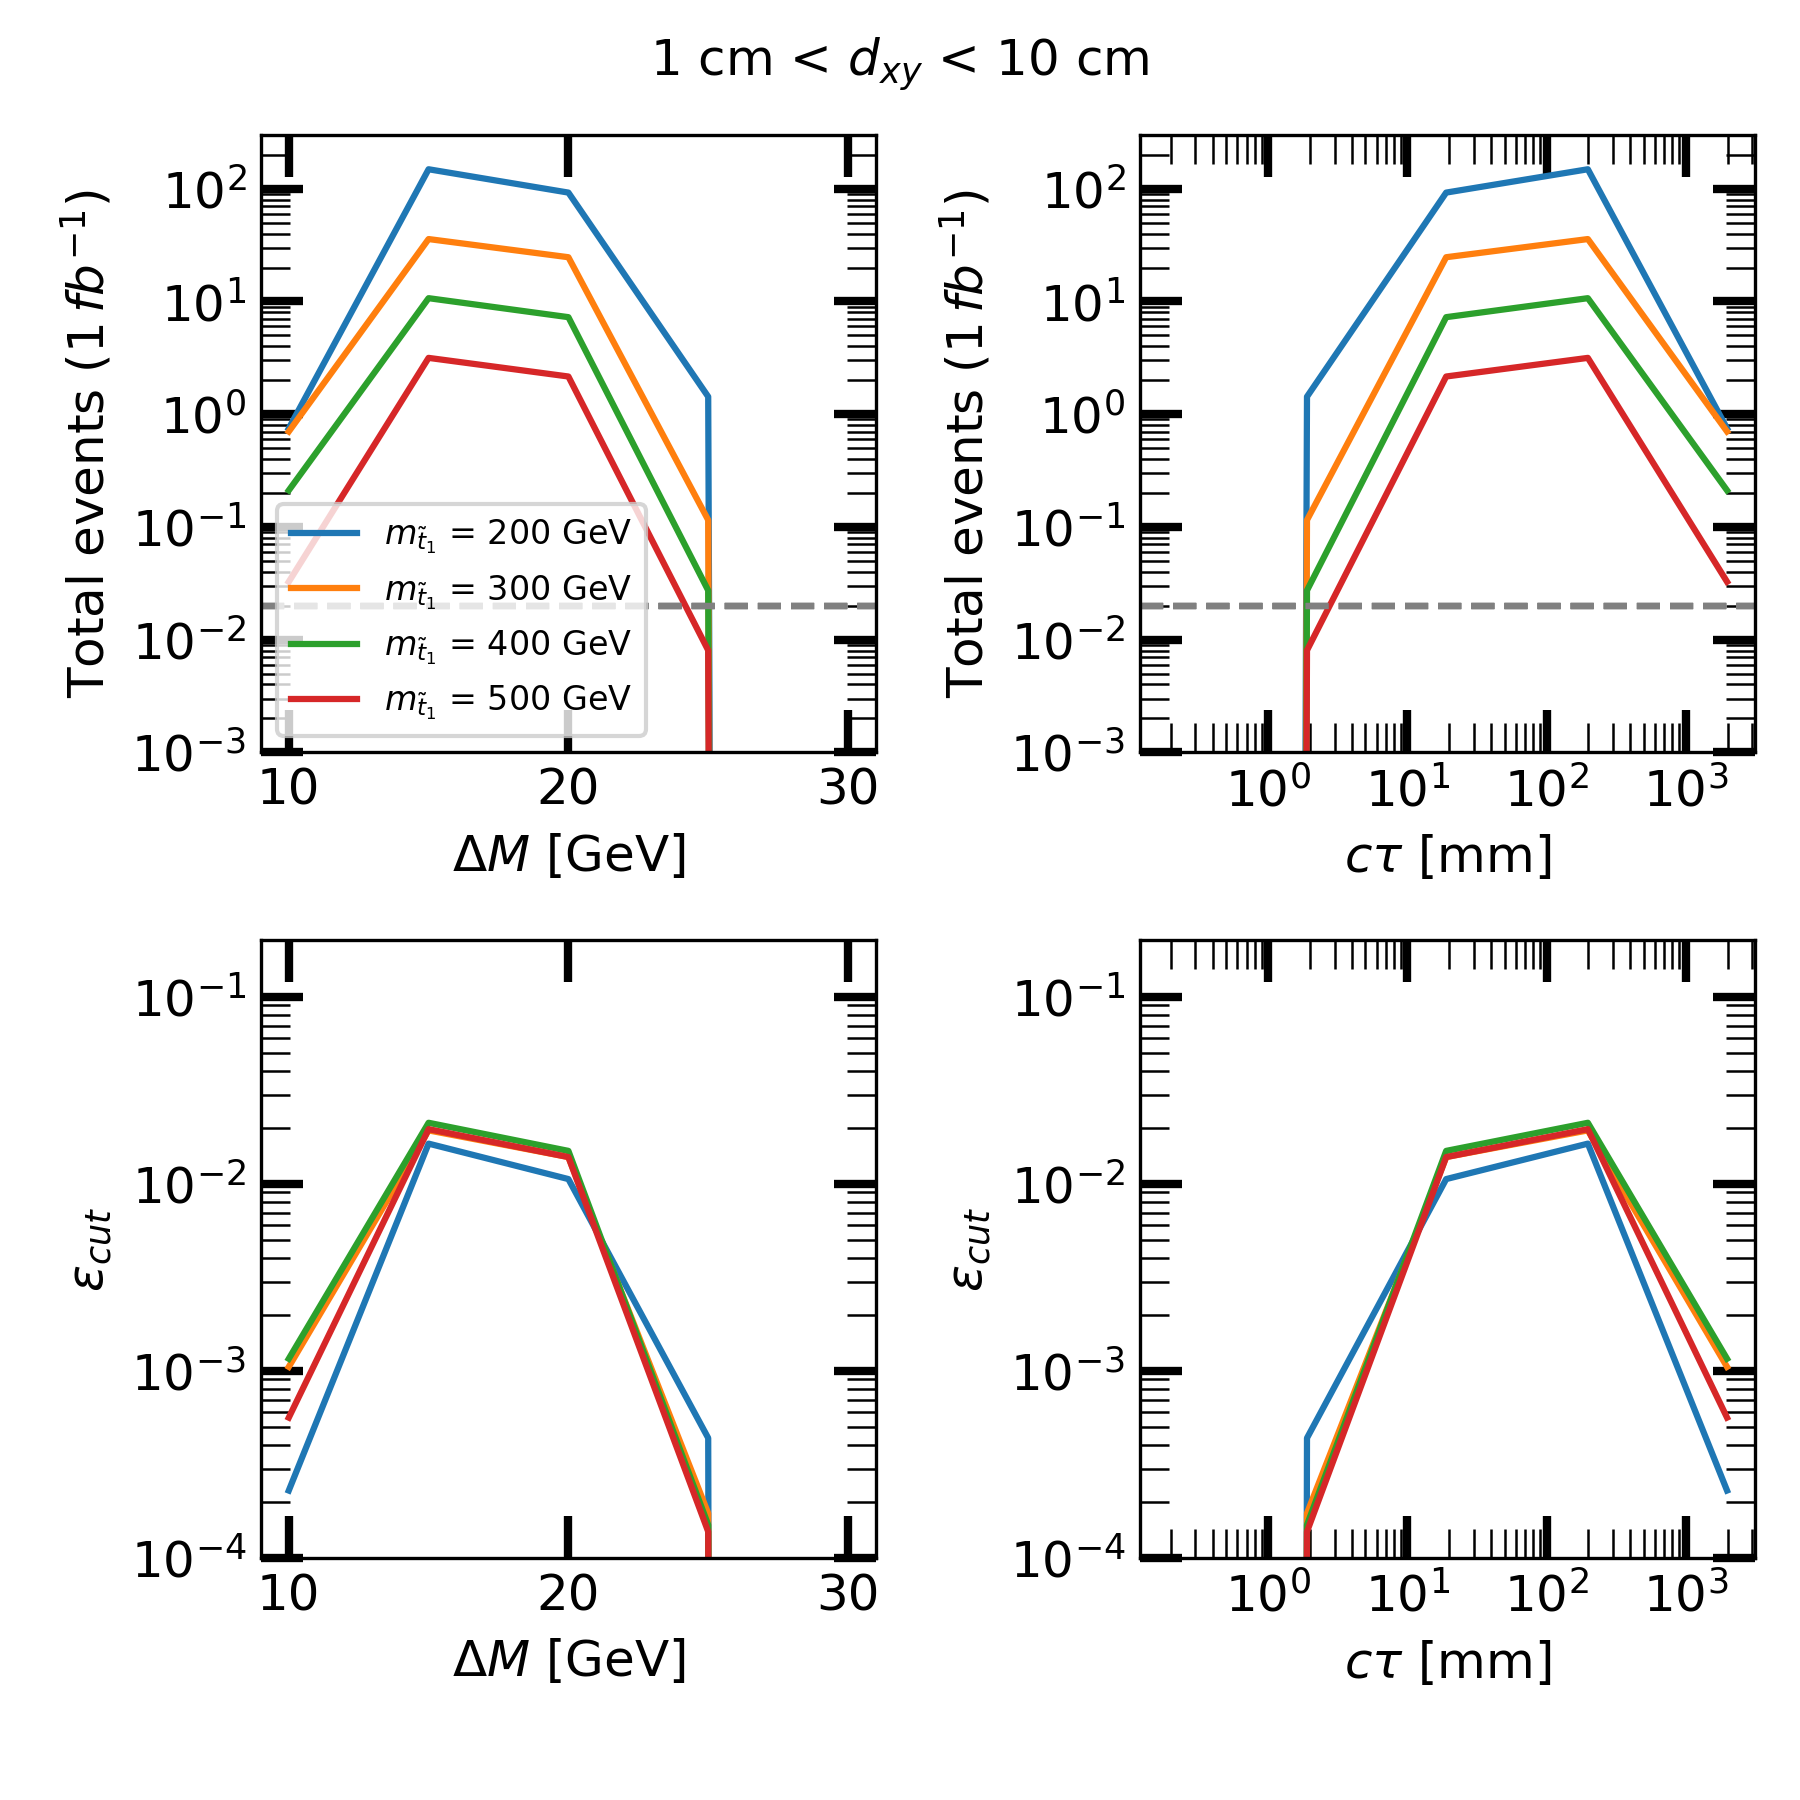
\includegraphics[width=0.8\columnwidth]{./figures/1_dxy_10_full_grid.png}%
 \caption{Same as above except for signal region $1 cm < d_{xy} < 10 cm$. }
\label{fig:full_grid_dxy10}
\end{figure}
%%%%%%%%%%%%%%%%%%%%%%%%%%%%%%%%%%%%%%%%%%%%%%%%%%%%%%%%%%%%

%%%%%%%%%%%%%%%%%%%s set ot%%%%%%%%%%%%%%%%%%%%%%%%%%%%%%%%%%%%%%%%%
\section{Lifetime reweighting}
\label{sec:lt}
%%%%%%%%%%%%%%%%%%%%%%%%%%%%%%%%%%%%%%%%%%%%%%%%%%%%%%%%%%%%
Given the true lifetime of sample $\tau_{\rm{true}}$, a new lifetime $\tau_{\rm{new}}$ can be obtained by constructing the ratio of PDFs with mean $\tau_{\rm{new}}$ and $\tau_{\rm{true}}$. The time $t$ at which the stop decays in the lab frame is obtained by 
\begin{equation}
    t = \frac{m}{p_T} \times L_{xy},
\end{equation}
where, $m$ is the mass of the decaying particle, here the stop, $p_T$ is the associated transverse momentum and the $L_{xy}$ is the displacement. Note, proper unit conversion is necessary in order to match units between $t$, here defined in units of length, and injected $\tau$, which may be in seconds depending on user settings. In the procedure followed, the injected liftetime is in mm and the computed $t$ is in cm, hence a factor of 10 in PDF appears when reweighting is performed. 

The weight of this stop is then computed by 
\begin{equation}
    w_i = \frac{\tau_{\rm{old}}}{\tau_{\rm{new}}}\times \frac{\exp ( -t/\tau_{\rm{new}})}{\exp ( -t/\tau_{\rm{old}})}.
\end{equation}

%%%%%%%%%%%%%%%%%%%%%%%%%%%%%%%%%%%%%%%%%%%%%%%%%%%%%%%%
\begin{figure}[tb]
%\subfloat{%
  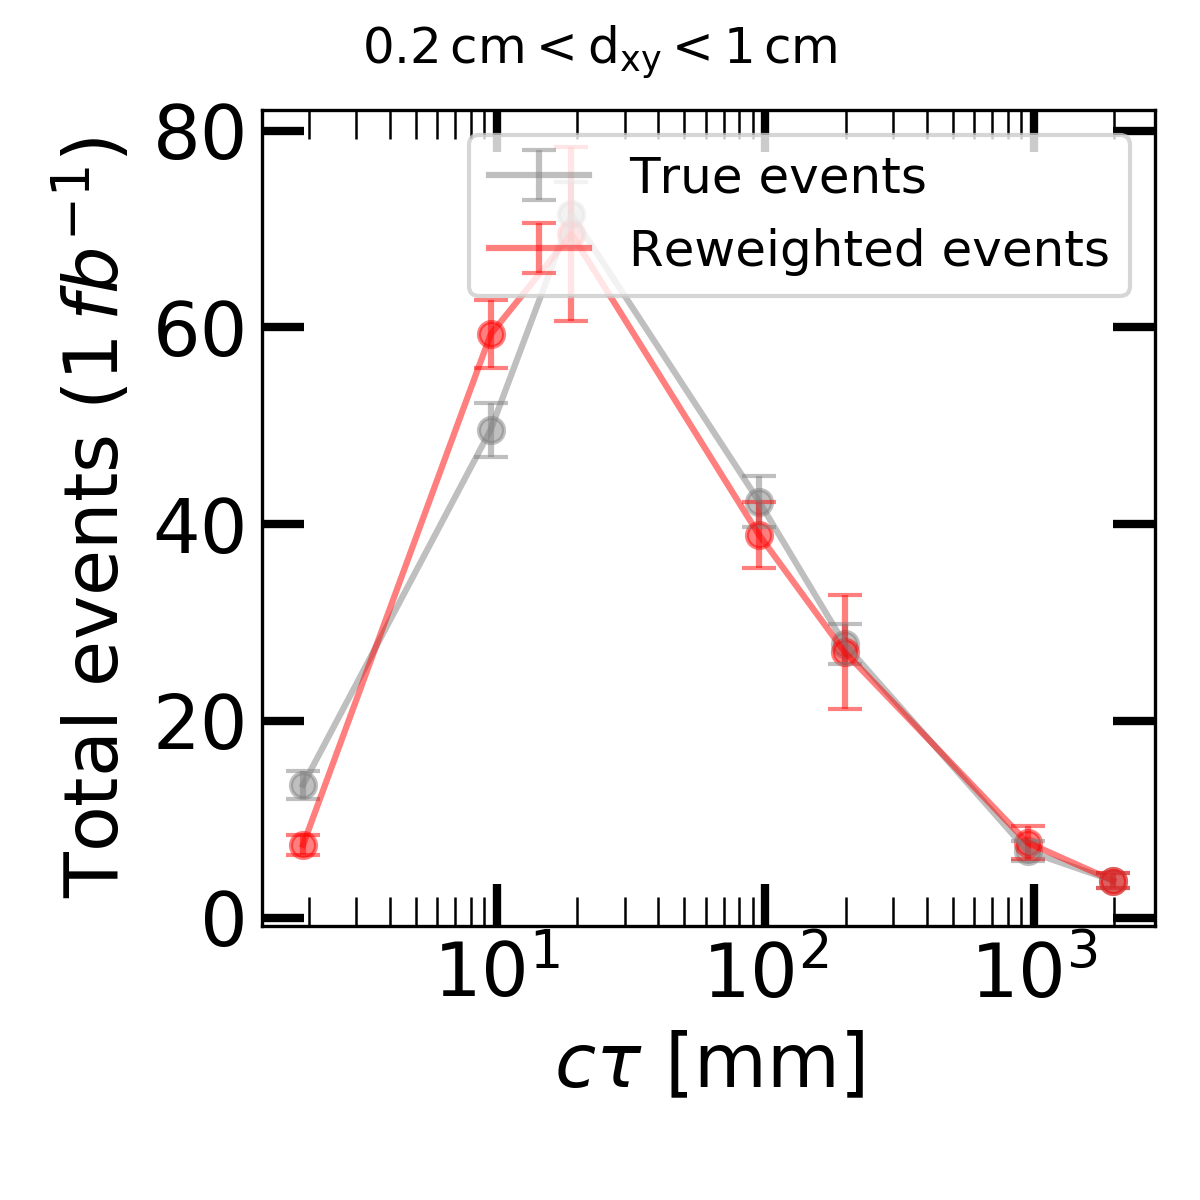
\includegraphics[width=0.45\columnwidth]{./figures/dxy_02_1_total_lt.png}%
  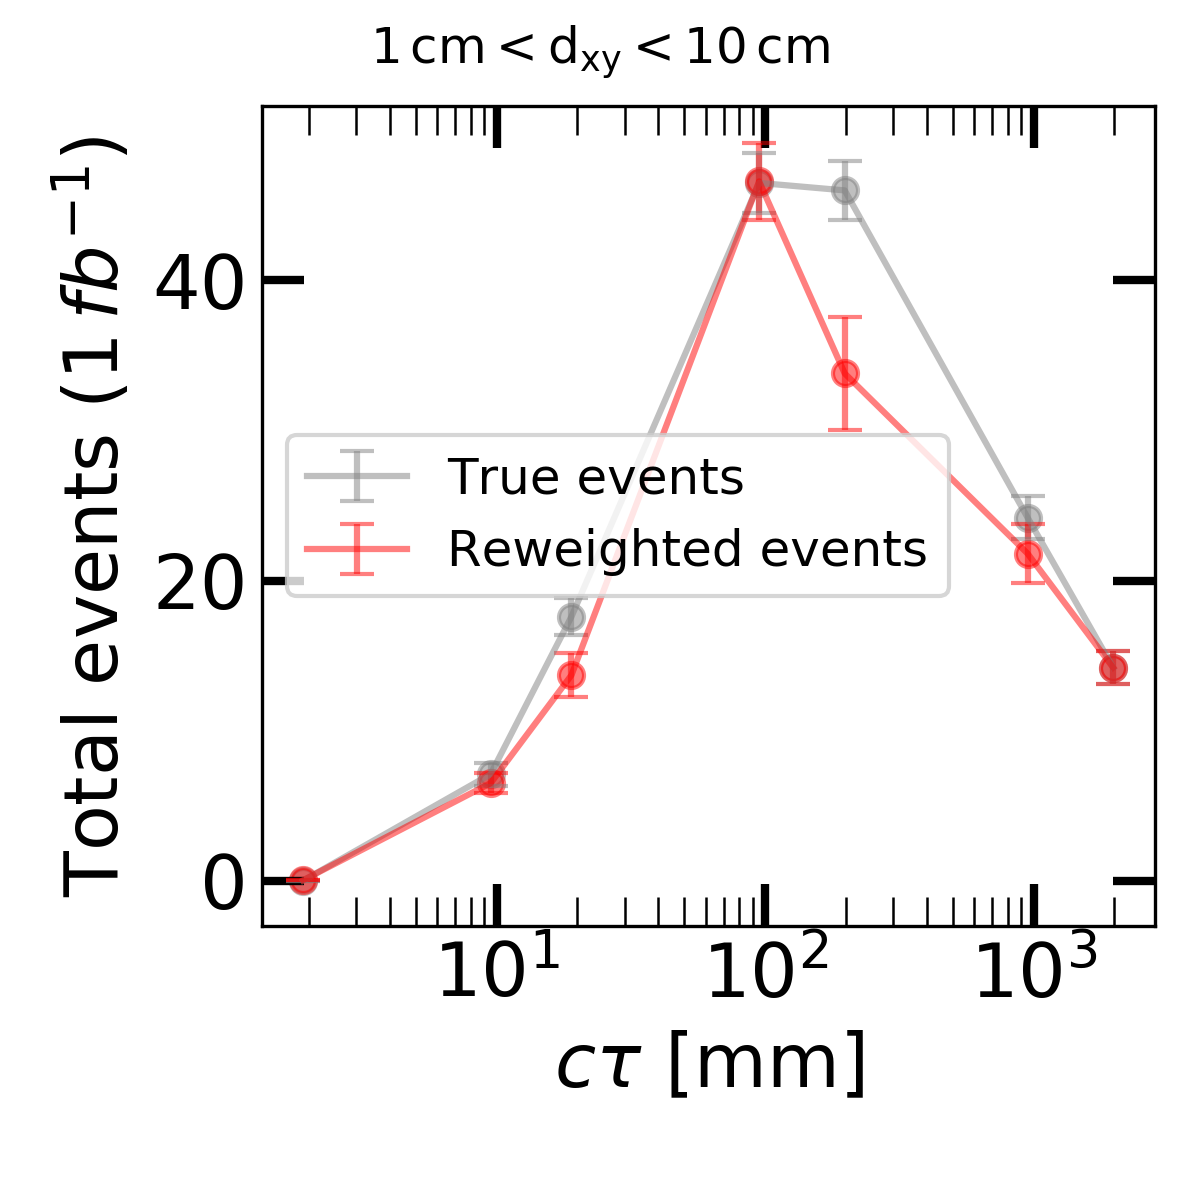
\includegraphics[width=0.45\columnwidth]{./figures/dxy1_10_total_lt.png}
 \caption{Reweighted events and true events as a function of lifetime for the grid as described in sec/~\ref{sec:lt}. To get the reweighted events (red line), the nearest larger lifetime sample is used. E.g. to get the numbers of 950mm of lifetime, true lifetime sample at 1980mm is used.  }
\label{fig:lt_reweight}
\end{figure}
%%%%%%%%%%%%%%%%%%%%%%%%%%%%%%%%%%%%%%%%%%%%%%%%%%%%%%%%%%%%

Since we need to reweight both legs of the stops, the final weight of the event is
\begin{equation}
w_{\rm{lt}} = w_1 \times w_2.
\end{equation} 

In order to perform the proof of principle exercise, a sample with six lifetimes was generated. These lifetimes were 1980mm, 950mm, 198mm, 95mm, 19mm, 9.5mm, 1.9mm. For each sample approximately 20 to 30k events after filter and matching were generated. Since the lifetime reweighting does not depend on the branching ratio, we use a four body branching ratio of 100\% in order to perform this exercise. 

In fig.~\ref{fig:lt_reweight}, we show the results of our reweighting exercise for the two signal regions under consideration as compared to the true events obtained. In order to obtain reweighted events, we take the nearest sample with a larger lifetime e.g. in order to obtain events for $c\tau = 950$mm, we use the sample with $c\tau = 1980$mm. We see that this procedure works rather well. 
%%%%%%%%%%%%%%%%%%%%%%%%%%%%%%%%%%%%%%%%%%%%%%%%%%%%%%%%%%%%
\section{Branching ratio reweighting}
\label{sec:br}
%%%%%%%%%%%%%%%%%%%%%%%%%%%%%%%%%%%%%%%%%%%%%%%%%%%%%%%%%%%%
The previous philosophy of reweighting being a ratio of PDF is also followed for reweighting branching ratios.

We are inters ted in obtaining a sample with four body branching ration $BR_4^{new}$ given true 4 body branching ratio sample $BR_4^{true}$. The PDF in branching ratio is a flat PDF and hence the weight of a stop decaying with 4 body final state is computed as: 
\begin{equation}
    w^4_i = \frac{BR_4^{new}}{BR_4^{true}}.
\end{equation}
%%%%%%%%%%%%%%%%%%%%%%%%%%%%%%%%%%%%%%%%%%%%%%%%%%%%%%%%
\begin{figure}[tb]
%\subfloat{%
  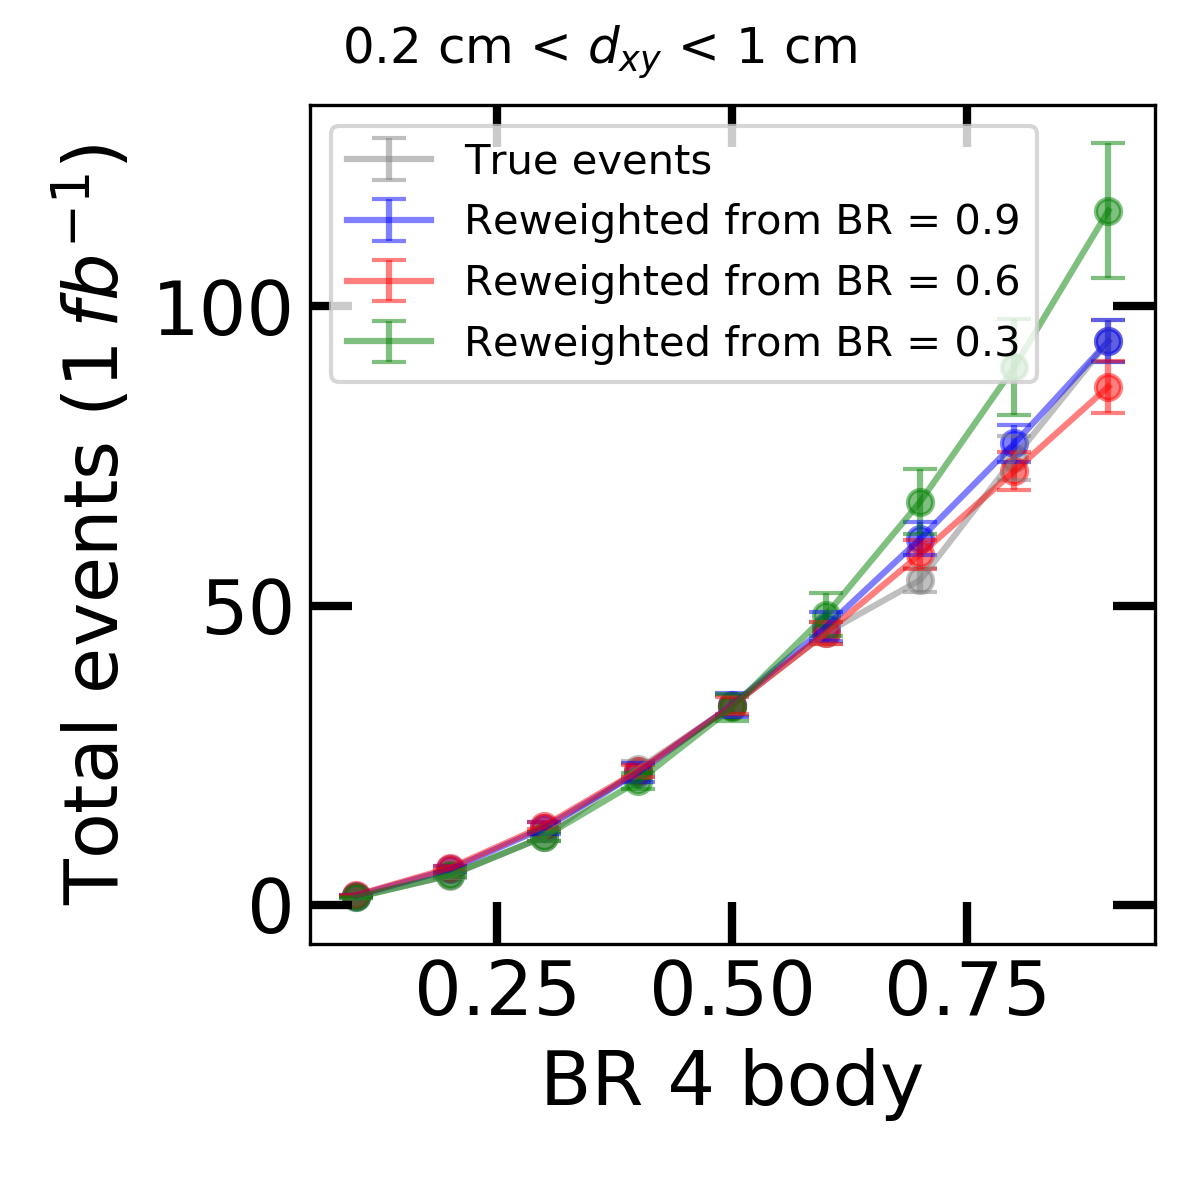
\includegraphics[width=0.45\columnwidth]{./figures/02_dxy_1_br.png}%
  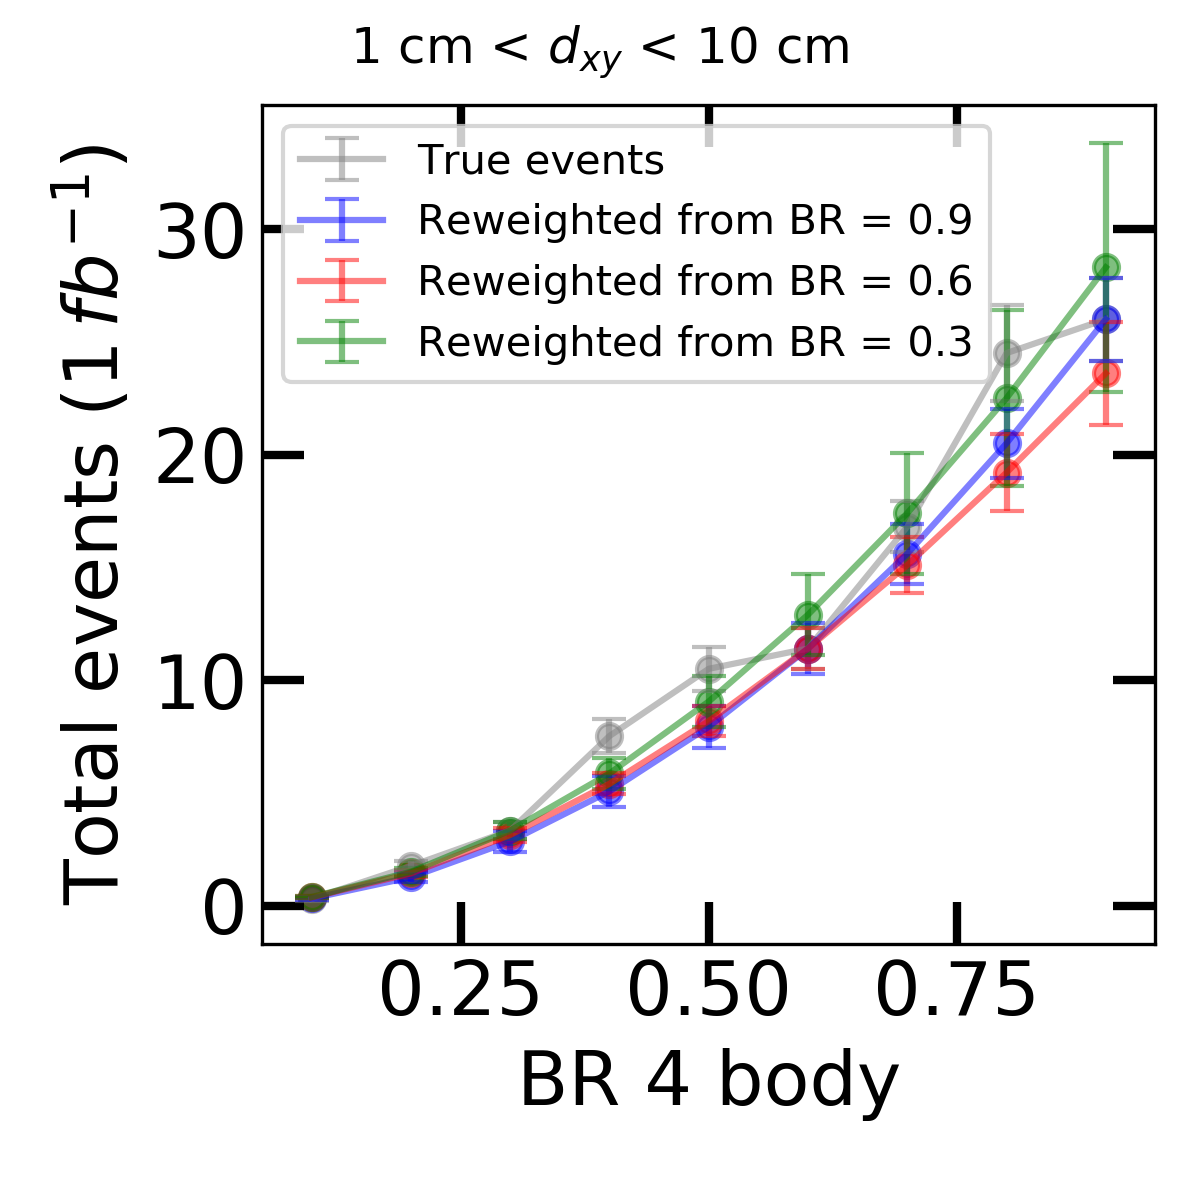
\includegraphics[width=0.45\columnwidth]{./figures/1_dxy_10_br.png}\\
  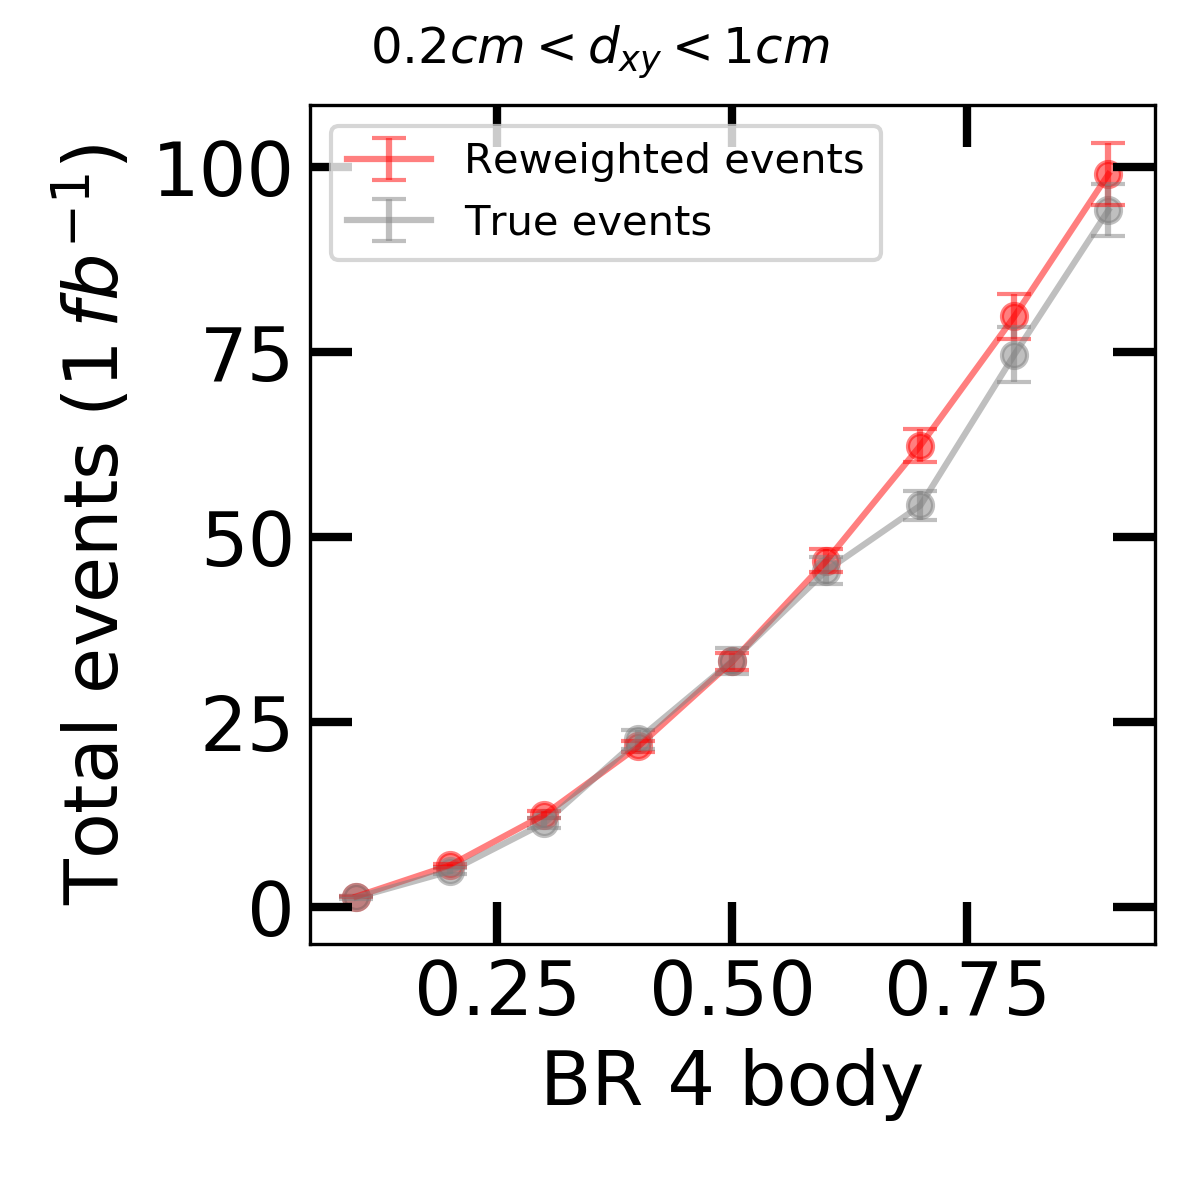
\includegraphics[width=0.45\columnwidth]{./figures/dxy_02_1_total_br.png}%
  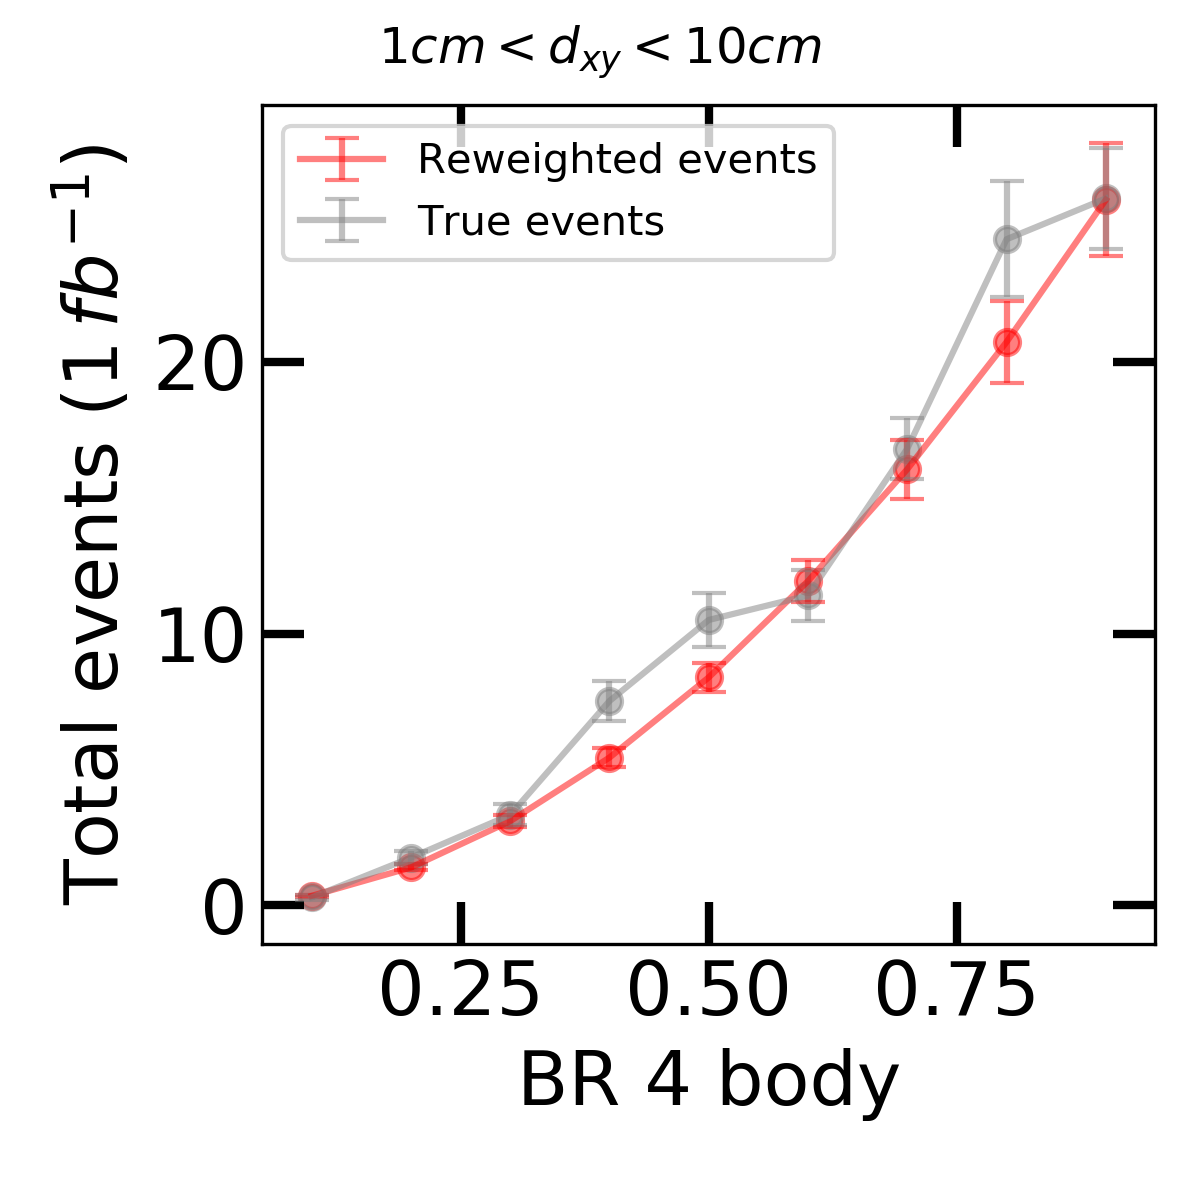
\includegraphics[width=0.45\columnwidth]{./figures/dxy1_10_total_br.png}%
 \caption{(Top row): True number of events and reweighted events as a function of 4-body branching ratio. The reweighted events are obtained from true BR of 0.3, 0.6 or 0.9. (Bottom row): True events and reweighted events as a function of 4-body BR. The reweighted events are obtained from a sum over all PDFs of 0.3, 0.6, 0.9 samples.}
\label{fig:br_reweight}
\end{figure}
%%%%%%%%%%%%%%%%%%%%%%%%%%%%%%%%%%%%%%%%%%%%%%%%%%%%%%%%
The corresponding two body branching ratio is hence: $1-BR_4$ and the weight is given by 
\begin{equation}
    w^2_i = \frac{1 - BR_4^{new}}{1- BR_4^{true}}.
\end{equation}
For each event depending on the stop final states, the appropriate weight is the multiplication of respective branching ration. For example for an event containing both stops decaying via 4 body final state, the weight of the event is $w_{br} = w^4_1 \times w^4_2$.

In fig.~\ref{fig:br_reweight}, we show the results of reweighting. First, we show the reweighted events obtained by using a true branching ratio sample of 0.3, 0.6 and 0.9. Along with this we also show reweighted events obtained by combining the three samples. We see that this procedure works rather well. 
%%%%%%%%%%%%%%%%%%%%%%%%%%%%%%%%%%%%%%%%%%%%%%%%%%%%%%%%%
%%
\section{Practical details}
%%%%%%%%%%%%%%%%%%%%%%%%%%%%%%%%%%%%%%%%%%%%%%%%%%%%%%%%%%%%
\begin{itemize}
    \item Injected BR as specified in file names always corresponds to four body final states
    \item path to samples \begin{verbatim} /eos/user/s/sukulkar/stop_samples/ \end{verbatim}
    \item The directory contains three folders, one for lifetime reweighting \begin{verbatim} lt_reweight, \end{verbatim} for branching ratio reweighting \begin{verbatim} br_reweight, \end{verbatim} and finally the samples correspoding to the full grid \begin{verbatim} full_grid. \end{verbatim}
    \item path to fragments \begin{verbatim} Workspace/DegenerateStopAnalysis/python/fragments/
    \end{verbatim}
    \item existing stop gridpacks \begin{lstlisting}
        /cvmfs/cms.cern.ch/phys_generator/gridpacks/2017/13TeV/madgraph/V5_2.4.2/sus_sms/LO_PDF/SMS-StopStop/v1/SMS-StopStop_mStop-XXX_slc6_amd64_gcc481_CMSSW_7_1_30_tarball.tar.xz  
    \end{lstlisting}
\end{itemize}
%%%%%%%%%%%%%%%%%%%%%%%%%%%%%%%%%%%%%%%%%%%%%%%%%%%%%%%%%%%%
\section{Open questions}
%%%%%%%%%%%%%%%%%%%%%%%%%%%%%%%%%%%%%%%%%%%%%%%%%%%%%%%%%%%%
\begin{itemize}
    \item I could not make lifetime reweighting work by summing over all PDFs, I don't understand why. 
    \item For branching ratio reweighting the over fluctuation at 0.4, 0.5 and 0.8 is not understood. This seems to remain irrespective of the number of events generated. 
    \item One needs to vary over the stop four body branching ratio in full model and reassess the sensitivity. This has not been done. 
    \item The reconstruction efficiency as a function of stop $L_{xy}$ as shown by Kaushik need to be integrated in the code.
\end{itemize}
%%%%%%%%%%%%%%%%%%%%%%%%%%%%%%%%%%%%%%%%%%%%%%%%%%%%%%%%%%%%
%\section{Numbers}
%%%%%%%%%%%%%%%%%%%%%%%%%%%%%%%%%%%%%%%%%%%%%%%%%%%%%%%%%%%%

%\begin{itemize}
%    \item Average matching efficiency 0.3
%    \item Average filter efficiency 0.1
%\end{itemize}
%Useful condor command
%\begin{lstlisting}
%    ./submitCondor.py --slc6 --queue workday --execFile ~/CMSSW_10_2_18/src/Analysis/Tools/scripts/condor.sh exe_cfg.sh 
%\end{lstlisting}
\bibliography{Refs}
\end{document}  